\section{Anomaly detection with generative models: practical example} \label{sec:alfven}
In this section, an application of generative modelling on a practical example is presented. It was previously published in~\cite{vskvara2020detection}. Some of the different generative autoencoders presented in Sec.~\ref{sec:vae_models} will be used to model data measured in a complex scientific experiment. Apart from the comparison of the previously presented anomaly scores, consider this to be a preliminary exploration of the two-stage modeling approach to anomaly detection described at the end of Sec.~\ref{sec:ad_genmodels}, where an autoencoding model is used to create a meaningful low-dimensional representation of complex data, and which is then coupled with some classical detector from Sec.~\ref{sec:taxonomy}. The same concept will also be further explored in Chapter~\ref{sec:chapter_sgvaegan}.

\begin{figure}[t]%[!htbp]
  \centering
  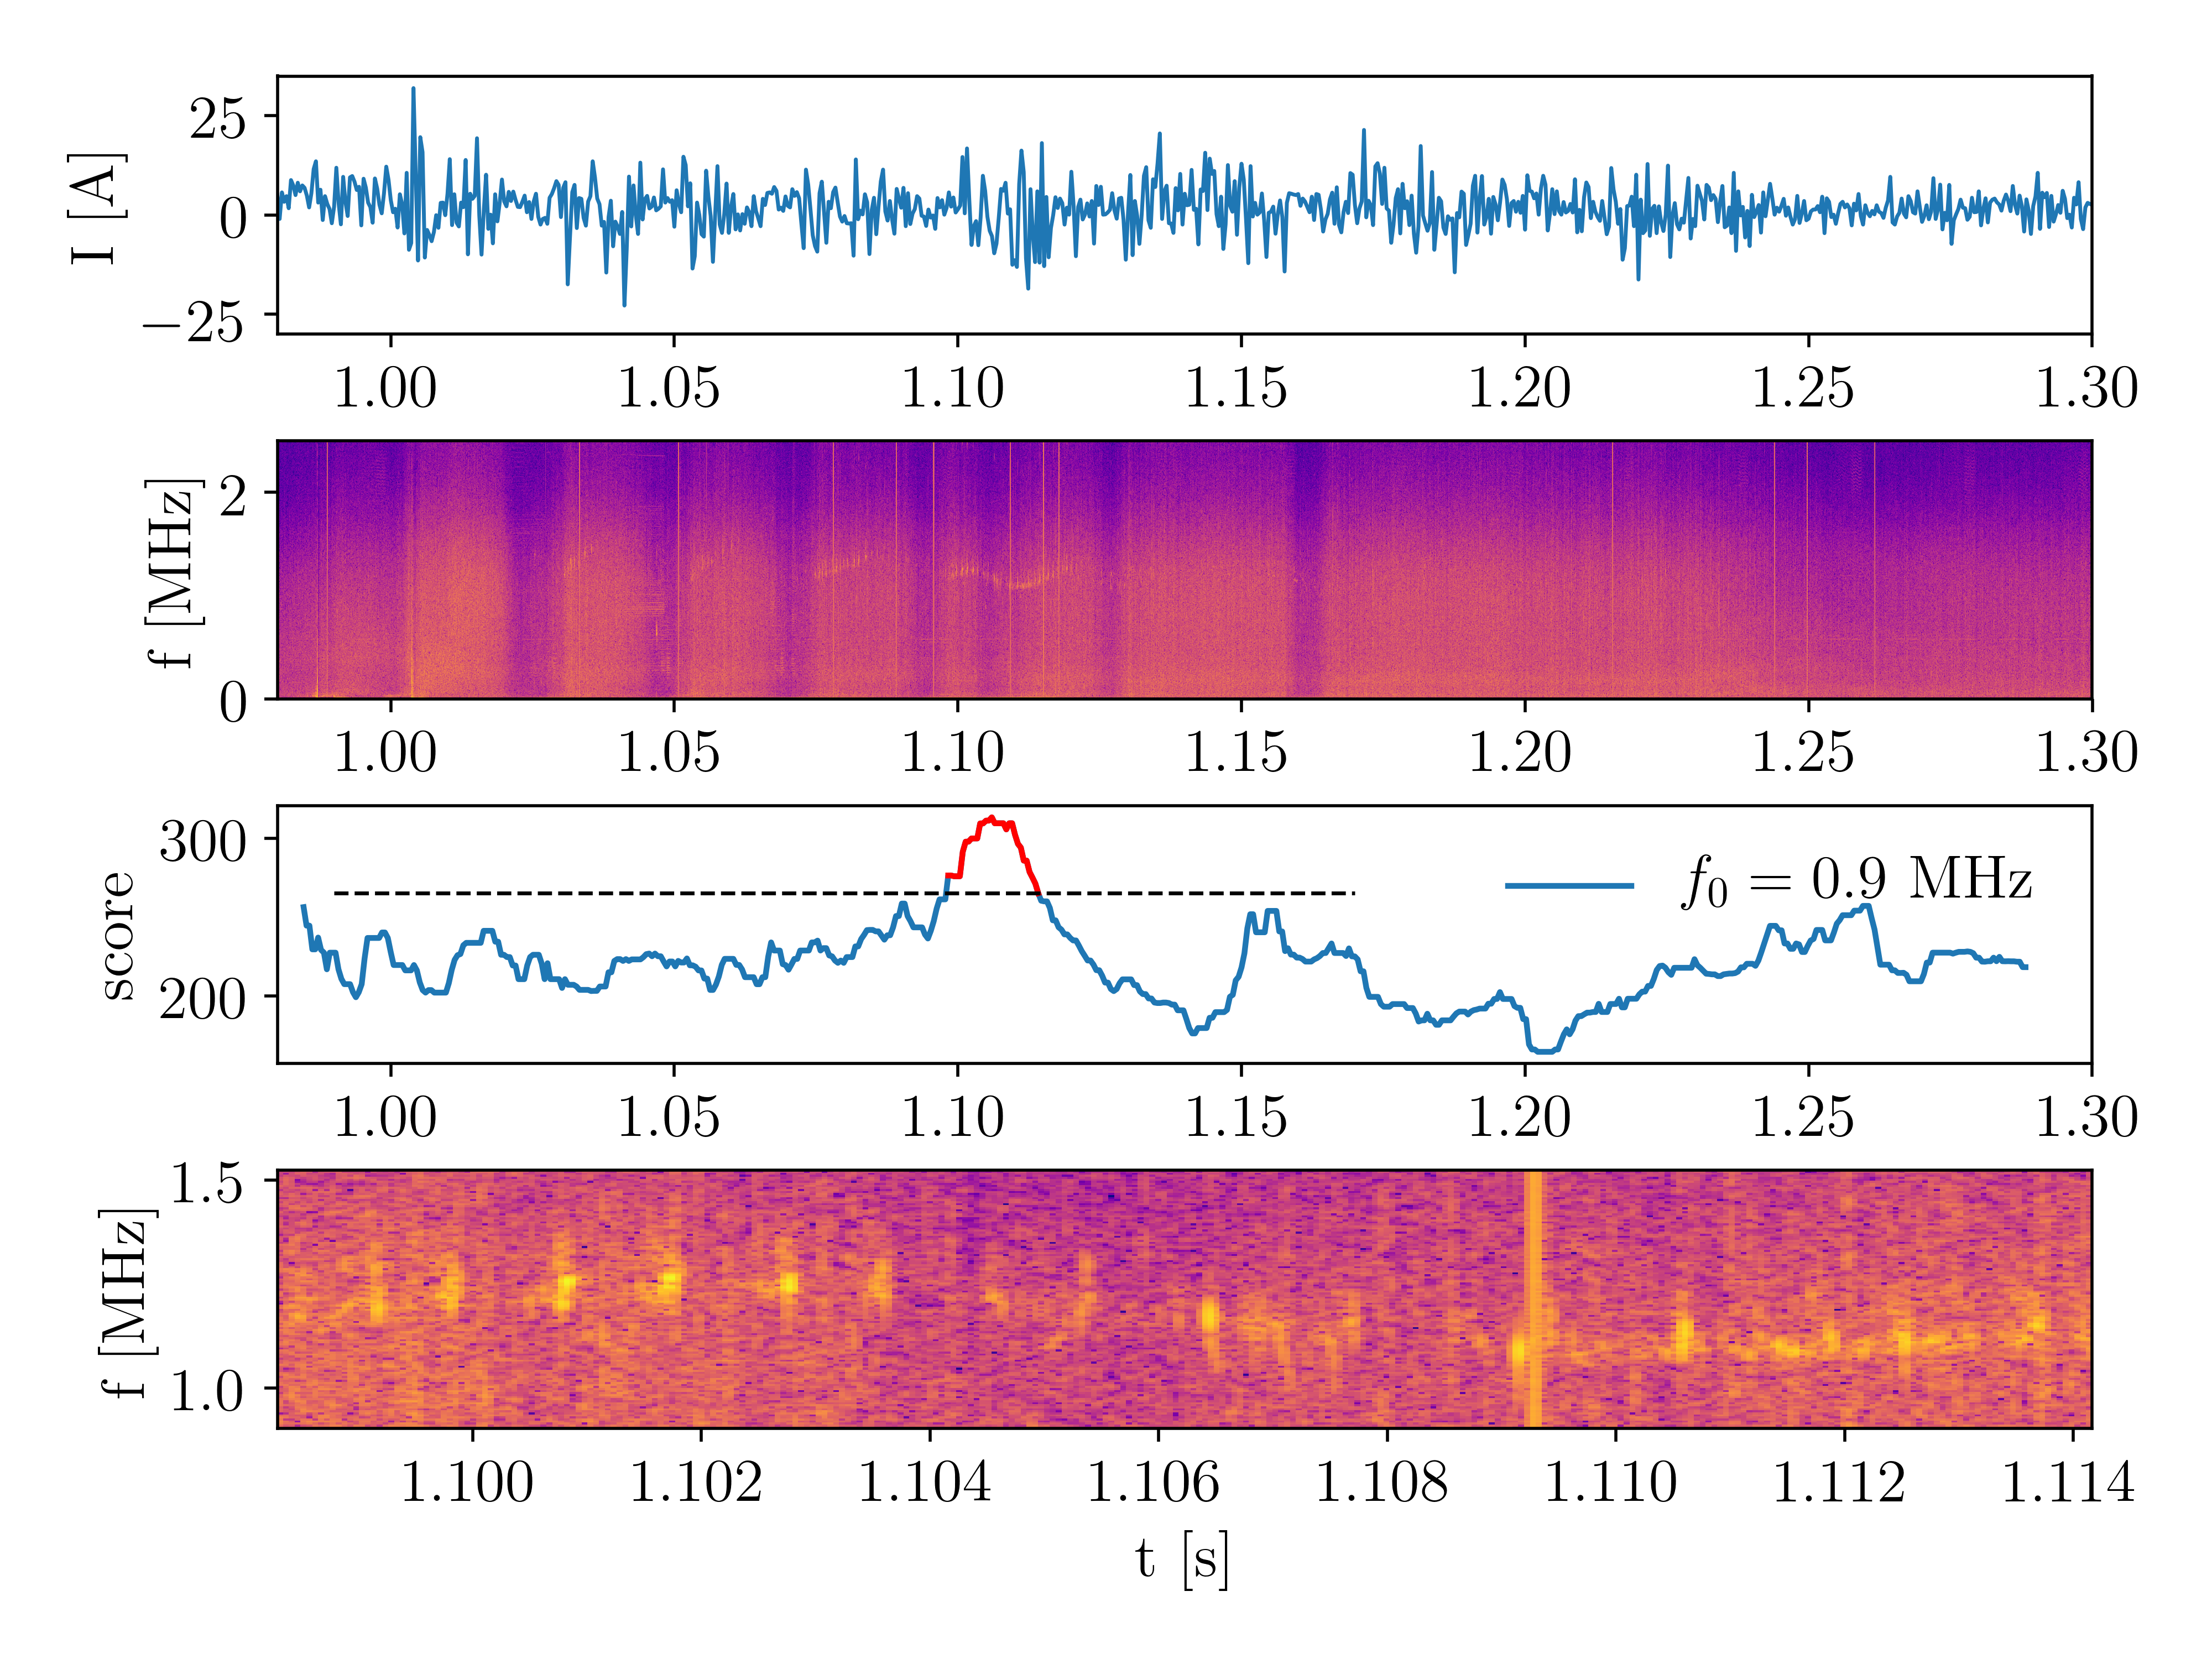
\includegraphics[scale=0.7]{data/chapter_alfven/overview.png}
  \caption{COMPASS shot 10870. Raw U-probe signal is in the upper plot. The corresponding spectrogram is below that. The score is the output of one of the tested models over the spectrogram at $f_0=0.9$ MHz and it is plotted third from the top. The highest peak around 1.1s corresponds to a detected chirping mode. A close-up of the spectrogram part containing the chirping mode as detected from the red part of the score plot is at the bottom. The size of the close-up is 128 $\times$ 311 pixels.}
  \label{fig:psd}
\end{figure}

\subsection{The application problem}
As already mentioned in the introductory chapter, physics has recently enjoyed an influx of very large amounts of data~\cite{bird2011computing,ball2010data} that needs to be processed and most importantly, from which new scientific discoveries may be extracted. This is also true for the field of plasma fusion, which pursues the goal of controlling a fusion reaction as a clean and almost inexhaustible source of energy. The ITER project~\cite{holtkamp2007overview}, which is going to be one of the largest and most complicated scientific experiments in history, is expected to produce up to 2 petabytes of data every day. This naturally calls for automatic processing of the data for a multitude of tasks, including anomaly detection. Currently, tokamaks are the state-of-the-art devices for experiments with controlled plasma fusion. In this section, an anomaly detection problem that appears during the operation of the COMPASS~\cite{panek2015status} tokamak will be dissected.

During the operation of COMPASS, \textbf{Alfv\'en eigenmodes}~\cite{markovic2015alfven, melnikov2015quasicoherent, markovic2017alfven} were observed. Alfv\'en eigenmodes are magnetic instabilities that degrade the performance of the tokamak and possibly endanger the plasma-facing components of the magnetic chamber~\cite{mett1992kinetic}. For this reason, their automatic detection is very important. Also, it may offer an opportunity for the study of their interactions with high-energy particles present in the plasma during an experiment. On COMPASS, chirping Alfv\'en eigenmodes are estimated to appear in about 0.1\% of all experiments. The primary means of their identification is a manual inspection of spectrograms drawn from the signal of certain magnetic probes, which is very time-consuming. See Fig.~\ref{fig:psd} for an example of the measured signal, a spectrogram that is derived from it, and a detected chirping Alfv\'en eigenmode. The spectrograms such as the one in Fig.~\ref{fig:psd} are large, so they are divided into patches of 128x128 pixels which is a feasible input size for current convolutional neural network architectures. It is also enough to capture most of a typical chirping mode as can be seen in the bottom plot in Fig.~\ref{fig:psd}. The patches that contain a chirping Alfv\'en eigenmode are considered to be anomalies. There are 370 labeled examples of patches with a chirping Alfv\'en eigenmode and a large database containing 33000 unlabeled (but considered normal) patches. This is a typical anomaly detection problem, where labeled anomalies are only used for evaluation and comparison of different models and the training dataset is considered to be anomaly-free.


\begin{figure}[ht]
\begin{center}
\begin{tikzpicture}[scale=1, transform shape]
  \vspace{-10cm}
  \node (image) at  (0,0) {\includegraphics[width=\linewidth]{data/chapter_alfven/model_structure.pdf}};
  \node (encdim) at (-6,\capy) {$\vc{x} \in \mathbb{R}^{128\times128\times1}$};
  \node (decdim) at (6,\capy) {$\vc{x}' \in \mathbb{R}^{128\times128\times1}$};
  \node (latdim) at (0, \capy) {$\vc{z} \in \mathbb{R}^{h}$};
  \node (enc) [align=left] at (\encx, .3) {$e_{\vc{\phi}}(\vc{x})$};
  \node (dec) [align=left] at (\decx, .3) {$g_{\vc{\theta}}(\vc{z})$};
\end{tikzpicture}
\end{center}
\caption{A schematic diagram of the convolutional autoencoder used for our experiments. Spectrogram patches are encoded through several convolutional, maxpooling and dense (fully connected) layers into $h$-dimensional vectors (here $h=2$) and then decoded back with transposed convolutions and upscaling layers.}
\label{fig:alfven_ae}
\end{figure}

\subsection{The experimental setup}
Two basic experimental setups are tested in this section. Both are based on generative autoencoders from Sec.~\ref{sec:vae_models}. The basic models have similar architectures, but they differ in the probability divergences used to regularize the latent space. The KLD~\eqref{eq:vae_kld} of a VAE model is compared against the MMD~\eqref{eq:mmd}. A WAE model with a discriminator is regularized by JSD which results in the training losses~\eqref{eq:aae_loss_disc} and~\eqref{eq:aae_loss_autoencoder}. Finally, a plain AE from Sec.~\ref{sec:reconstruction_models} is included to verify that a regularized latent space is useful. The individual components of the models (encoders, decoders, discriminators) are represented by neural networks with convolutional architecture. This is the most often used architecture for image data, as several levels of convolution operations are designed to capture shift-invariant features at different scales of an image. For more technical details on the construction of the models, see~\cite{vskvara2020detection}. A schematic of a prototypical model is in Fig.~\ref{fig:alfven_ae}. The models have Gaussian encoders and decoders. The prior is either $\mathcal{N}(0,\mathbf{I})$ or Vamp, as described in Sec.~\ref{sec:wae}, and the choice is treated as a hyperparameter. Note that Vamp is only possible to use with the MMD or JSD metrics or their combination.

In the first setup, the described models are compared against each other as primary anomaly detectors in the \textbf{one class} setting. This means that they are trained on the (assumed) normal spectrogram patches and the anomaly score is the sampled reconstruction error~\eqref{eq:score_sample} in case of probabilistic autoencoders, and the reconstruction error~\eqref{eq:ae_objective} in case of the plain autoencoder model. This will test the proposed robustness of generative autoencoders.

In the second setup, the encoding capabilities of generative encoders are leveraged to create uncorrelated low-dimensional representations of spectrogram patches. This is combined with a classifier in a combined \textbf{two-stage} model. The first stage is a convolutional generative autoencoder trained with unlabeled data. Through the use of MMD or $\text{JS}_D$ measures and Vamp, a separation of the encoded data into clusters that contain similar inputs can be enforced, which makes the task of the classifier easier. The second stage is a classifier that is trained on encoded labeled data. Two different classifiers were tested. The kNN classifier, which is similar to the kNN anomaly detector described in Sec.~\ref{sec:distance_methods}, and where the score of a sample is the average label of its $k$-nearest neighbors, assuming that the label $y \in \lbrace 0,1 \rbrace$ is zero for normal samples. The GMM classifier with $M$ components was fitted on the latent representations of both labeled and unlabeled training data. Afterward, we determine one or more components of the mixture into which the positively labeled training samples are most likely to be projected via the encoder. Then, for a new sample, the score is the (average) log-likelihood of the sample in the anomalous components. 

For more details on model architecture and hyperparameters used in the experiments, see~\cite{vskvara2020detection}. For both experimental setups, 10-fold cross-validation over different splits of training and testing data was done. In the experimental results below, the models are selected using average performance on the test set. This is not ideal, as will be shown in Chapter~\ref{sec:chapter_comparison}, but here the very low number of labeled anomalies would lead to nonrobust results if the proper train/validation/test split was done, which is even more pronounced by the splitting procedure described in Sec.~\ref{sec:alfven_splits}.

\subsection{Results}
\begin{figure}
\begin{centering}
\includegraphics[scale=0.5]{data/chapter_alfven/anomalies.png}
\par
\end{centering}
\caption{Examples of spectrogram patches identified as containing a chirping
mode.}
\label{fig:alfven_patches}
\end{figure}

During the use of one of the proposed models in the production environment of the tokamak, the following workflow would be observed. A set of experiments to be analyzed would be selected. Then, the needed signals would be extracted, spectrograms computed, and divided into patches of appropriate size. These would be fed to a trained model that would produce scores to enable a ranking of the patches. Since this would produce thousands of patches and scores for each tokamak experiment, the operator would ideally only want examine a few with the highest score. The problem is illustrated in Fig.~\ref{fig:alfven_patches}, where the output of such a procedure using one of the best-performing models is shown. It contains 4 patches with the highest score, out of which 3 contain a chirping mode. It illustrates that even though the neural network encoding might be powerful, it is still basically a black box model and we need to be very careful in its evaluation. Because of this, we evaluate the model performance not only by AUC~\eqref{eq:auc}, and also by the precision@$n$ score, which is the precision at the $n$-highest scoring samples, and which is useful because it can be tuned to a certain $n$ given by the operating conditions of the tokamak. Here, we use $n=50$, which is a realistic number of samples that an operator can examine for each tokamak experiment.

\begin{table}
  \centering
  \begin{tabular}[h]{c c c c} 
divergence & target class & AUC & precision@50 \\ 
\hline 
-- & Alfv\'en & $0.57 \pm 0.04$ & 0.24 $\pm$ 0.05 \\ 
KLD & Alfv\'en & 0.74 $\pm$ 0.06 & 0.44 $\pm$ 0.13 \\ 
MMD & Alfv\'en & 0.77 $\pm$ 0.03 & 0.49 $\pm$ 0.06 \\ 
JSD & Alfv\'en & 0.69 $\pm$ 0.07 & 0.42 $\pm$ 0.08 \\ 
MMD + JSD & Alfv\'en & 0.72 $\pm$ 0.09 & 0.37 $\pm$ 0.03 \\
-- & non--Alfv\'en & 0.82 $\pm$ 0.03 & 0.86 $\pm$ 0.06 \\ 
KLD & non--Alfv\'en & 0.46 $\pm$ 0.05 & 0.50 $\pm$ 0.14 \\ 
MMD & non--Alfv\'en & 0.84 $\pm$ 0.03 & \textbf{0.90 $\pm$ 0.06} \\ 
JSD & non--Alfv\'en & 0.84 $\pm$ 0.05 & 0.83 $\pm$ 0.10 \\ 
MMD + JSD & non--Alfv\'en & \textbf{0.84 $\pm$ 0.01} & 0.87 $\pm$ 0.01 \\ 
\end{tabular}

  \caption{Results of optimization of the one class model by the divergence used in latent space regularization. The top three values are highlighted with shading. No divergence is used in a plain autoencoder with the training objective~\eqref{eq:ae_objective}.}
  \label{tab:one_class}
\end{table}

Tab.~\ref{tab:one_class} compares the performance of models in the one-class setup. The results are split by the divergence used to regularize the latent space. The difference between MMD, JSD, and their combination in terms of AUC is negligible, but MMD is slightly better than the rest in terms of precision@50. Surprisingly, vanilla VAE with KLD fails in this task altogether, which indicates that the distribution of the patches with Alfvén eigenmodes is difficult to model through a latent space with a unimodal prior.

\begin{figure}
\begin{centering}
\includegraphics[scale=0.6]{data/chapter_alfven/roc_prc.pdf}
\end{centering}
\caption{ROC and PR curves of selected models. For brevity, we include the best one-class and best two-stage models in the same plot, although they are not directly comparable.}
\label{fig:roc_prc}
\end{figure}

\begin{table}
\centering
\begin{tabular}{c c c c}
	\toprule
	divergence & classifier & AUC & precision@50  \\
	\midrule
	-- & kNN & 0.80$\pm$0.07 &  \cellcolor{gray!15} 0.88$\pm$0.10 \\
	KLD & kNN & 0.80$\pm$0.08 & 0.85$\pm$0.11 \\
	MMD & kNN &  \cellcolor{gray!45} 0.91$\pm$0.06 &  \cellcolor{gray!45} 0.94$\pm$0.05\\
    JSD & kNN &  \cellcolor{gray!15} 0.83$\pm$0.07 & 0.87$\pm$0.10\\
    MMD + JSD & kNN &  \cellcolor{gray!30} 0.86 $\pm$ 0.07 &  \cellcolor{gray!30} 0.91$\pm$0.10 \\
    -- & GMM & 0.75$\pm$0.06 & 0.80$\pm$0.10\\
	KLD & GMM & 0.74$\pm$0.06 & 0.83$\pm$0.11\\
	MMD & GMM & 0.66$\pm$0.12 & 0.72$\pm$0.12\\
    JSD & GMM & 0.74$\pm$0.06 & 0.82$\pm$0.11\\
    MMD + JSD & GMM & 0.76$\pm$0.06 & 0.84$\pm$0.10 \\
    \bottomrule
\end{tabular}
\caption{Results of hyperparameter tuning of the two-stage model across 10 cross-validation splits.}
\label{tab:alfven_results}
\end{table}

The performance of the two-stage models is summarized in Tab.~\ref{tab:alfven_results}. What is immediately obvious is that the simple kNN model is superior to the GMM approach with any encoding. Also, MMD regularization produces the best results. We might speculate that this might be due to the improved ability to produce a well-separated encoding enforced by the used prior. Fig.~\ref{fig:roc_prc} captures the ROC and PR curves for the best one-class and two-stage models.

A question one might ask is whether the use of an autoencoder is truly necessary. In the end, we are doing a projection from $d=128\times128=16384$ dimensional picture space into at most $h=64$ dimensional latent space which must naturally lead to a loss of information. As shown in Fig.~\ref{fig:patches_latent}, where $h=8$, the autoencoder is able to identify the difficult nonlinear correlations and improve the performance of a subsequent second-stage kNN model. The compression is clearly necessary for overcoming the curse of dimensionality which says that the L$_2$ distance degenerates in large dimensions. An alternative approach to overcoming the issue of large input dimension might be to train a classification convolutional neural network, which does the compression by its nature. However, such a network would be highly susceptible to overfitting since it requires a lot of labeled data that is not available.

\begin{figure}
\centering
\includegraphics[scale=0.45]{data/chapter_alfven/split_patches.pdf}
\includegraphics[scale=0.45]{data/chapter_alfven/split_spectrograms.pdf}
\caption{kNN fits for different values of $k$. The red line and band show the mean and one standard deviation bands of the resulting AUC values when kNN is fitted to the original vectorized images. The input space dimensionality is $h=16384$. The blue dashed line and band are the same quantities for a $h=8$ dimensional representation by a first-stage model. On the left, the training and testing splits were done on the level of individual patches, leading to improved performance and less variance. On the right, the split was done on the level of the original spectrograms, which is a more realistic scenario. The standard deviation and mean were computed from 10 random splits.}
\label{fig:patches_latent}
\end{figure}

\subsubsection{Influence of the train/test splitting methodology} \label{sec:alfven_splits}
At first, the splitting of testing and training labeled patches was done on the level of patches, without any regard for the spectrogram/experiment that the patch came from. It was assumed that the labeled chirping modes are homogeneous across the spectrograms. However, this turned out not to be true. Therefore, the train/test splits were done on the level of spectrograms which were then subsequently divided into patches. See Fig.~\ref{fig:patches_latent} where on the left side, the AUC curves for different values of $k$ of the kNN model are for the case when the data split was done on the level of patches. The blue line that is the result of a kNN fit peaks at $k=3$. On the other hand, there is no such peak on the right side of the figure, where splitting was done on the level of spectrograms. This indicates that the positively labeled patches in a single spectrogram are much more similar to each other than to those in different spectrograms, as only a relatively low number of neighbors is sufficient for optimal performance. Also, the variance of the right-side plots is much higher, again indicating larger differences across spectrograms. If we continued with the splitting on the level of patches, we would have a biased and too optimistic estimate of performance before using the framework in a production environment.

\subsubsection{Final remarks}
To sum up the findings from this section: generative autoencoders are a viable tool for unsupervised and semi-supervised anomaly detection. The information contained in the latent spaces is useful for anomaly detection, provided we have at least some examples of labeled anomalies. And finally, the kNN classifier proved to work very well in this simple experiment. All of these findings are going to be useful in the building of the model that is presented in Chapter~\ref{sec:chapter_sgvaegan}. 